\documentclass{article}
\usepackage{graphicx}
\graphicspath{ {images/} }
\begin{document}
\noindent Emily Mulhall\\
COMP 551 section 002\\
Assignment 1\\
January 29th, 2018\\

\section*{Question 1}
\begin{enumerate}
\item The training error is approximately 7.169 and the valid error is approximately 336.555
The fit on the training data is as follows:\\
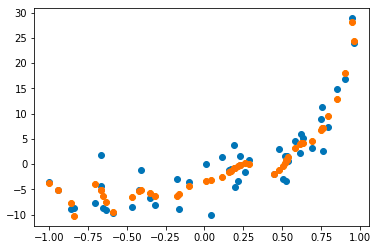
\includegraphics{trainerr1}
The fit on the valid data is as follows:\\
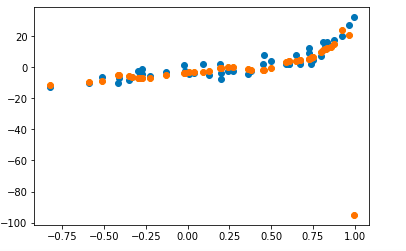
\includegraphics{validerr1}

Overall, the fit does closely resemble the trend of the data.  However, due to the noise in the data, the fit often has predictions that are more in the smooth than the actual data.  I am very confused by the outlier in the valid data at the x value of 1.  It seems to completely contradict the trend of the data at that point.

\item The error with the regularization with the lambda value of 0.01 has a training error of approximately 8.812 and a testing error of approximately 10.841.\\

The fit on the training data is as follows:\\
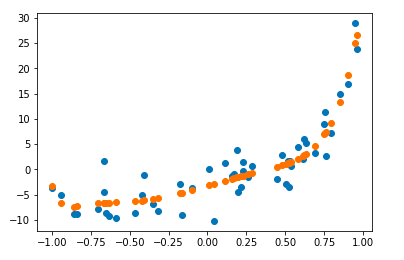
\includegraphics[width=9cm, height=5cm]{trainerr1b}\\
The fit on the testing data is as follows:\\
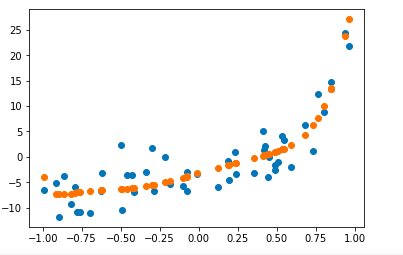
\includegraphics[width=9cm, height=5cm]{testerr1b}\\
The fit is now far smoother than in the graphs above which do not use regularization in the regression model.  Though the error is slightly higher in the training, the test error is far more reasonable than the valid error was in 1a.  Without regularization the model was clearly overfitting on the training data.  With regularization the fit is far more reasonable and generalizable.
\item I believe that the polynomial is likely of degree 4.  Looking at the graphs above the trend has a slightly parabolic shape, but the left side is far lower than the right side, which leads me to believe that the polynomial is of an even degree that is higher than 2.  The next logical guess is thus a degree of 4.  However, many higher order even polynomials could have a similar shape, and thus it is possible that the degree is actually slightly higher than 4.
\end{enumerate}
\section*{Question 2}
\begin{enumerate}
\item  The first graph is the training error over epochs and the second is the valid error over epochs:\\
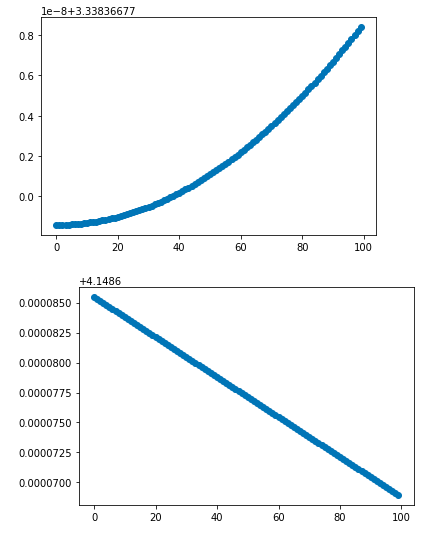
\includegraphics[width=9cm]{train_valid2a}\\

It is clear from these two graphs that as the epochs increase, the training error increases.  However, as they increase the valid error actually decreases.  This shows that as the stochastic gradient descent continues the fit is becoming less overfitted to the training data and becoming more generalizable.
\item In order to test different step sizes I went from a step size of 1e-6 to 1e-4 by an increment 1e-7.  Because of the computational time of this I reduced the number of epochs to 20.  I found that the step size of 9.9e-6  had the lowest error of 3.74351046565.  When run over 100 epochs with the step size of 9.9e-6 the test error rate was 3.61813316037. 

\item The below image shows the progression throughout 100 epochs:\\
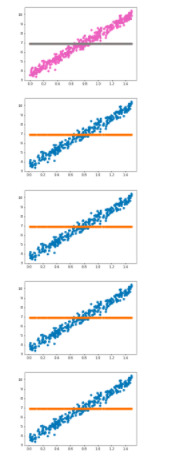
\includegraphics[width=10cm, height=20cm]{epochs}\\

Though it is difficult to see from the graphs, the error decreases over epochs from 3.61829601168 to 3.61813316037.
\end{enumerate}
\section*{Question 3}
\begin{enumerate}
\item See dataset handed in on MyCourses.
\item The MSE of the best fit on the testing data is 0.01989083.  Most parameters were learned except for the parameters represented by the first 4 columns.  The names of the cities had already been removed from the data, so that parameter was not learned.  The first 4 columns represent information about the location of the community, and therefore are not important in the learning.
\item \begin{tabular} {c c c}
Lambda Value & Training MSE & Test MSE\\
0 & 0.0156 & 0.01989\\
0.1 & 0.0157& 0.01960\\
0.2 & 0.01575& 0.01950\\
0.3 & 0.0158& 0.01945\\
0.4 & 0.01584& 0.01941\\
0.5 & 0.0159&0.01939\\
0.6 & 0.01592&0.01936\\
0.7 &0.0160&0.01935\\
0.8 & 0.0160&0.01934\\
0.9 &0.01602&0.01932\\
\end{tabular}\\


The above table shows different values for lambda in regularization and the training and testing error that results.  The optimal value for lambda is 0.4.  Because the information about the location of the community has very little weight given to its parameters, it is possible to use this information for feature selection.
\end{enumerate}
\end{document}